\section{Resultados}
Como resultados del prototipo, logramos regar una planta de lentejas utilizando Agrocare, también, como fruto de la investigación recolectamos data de 20 plantas que comúnmente se cultivan en huertos urbanos (Lentejas, Frijoles, Rábanos, Caléndula, Girasoles, Lechuga, Albahaca, Cactus, Orégano, Pimiento, Trigo, Avena, Centeno, Ajo, Guisantes, Lavanda, Tomillo, Margaritas, Claveles, Zanahoria) entre los datos recolectados se encuentra el estrés y déficit hídrico, qué condiciones de luminocidad y temperatura requieren, y qué cuidados especiales requieren.

\renewcommand{\figurename}{Figura}
\begin{figure}[h]
  \centering
  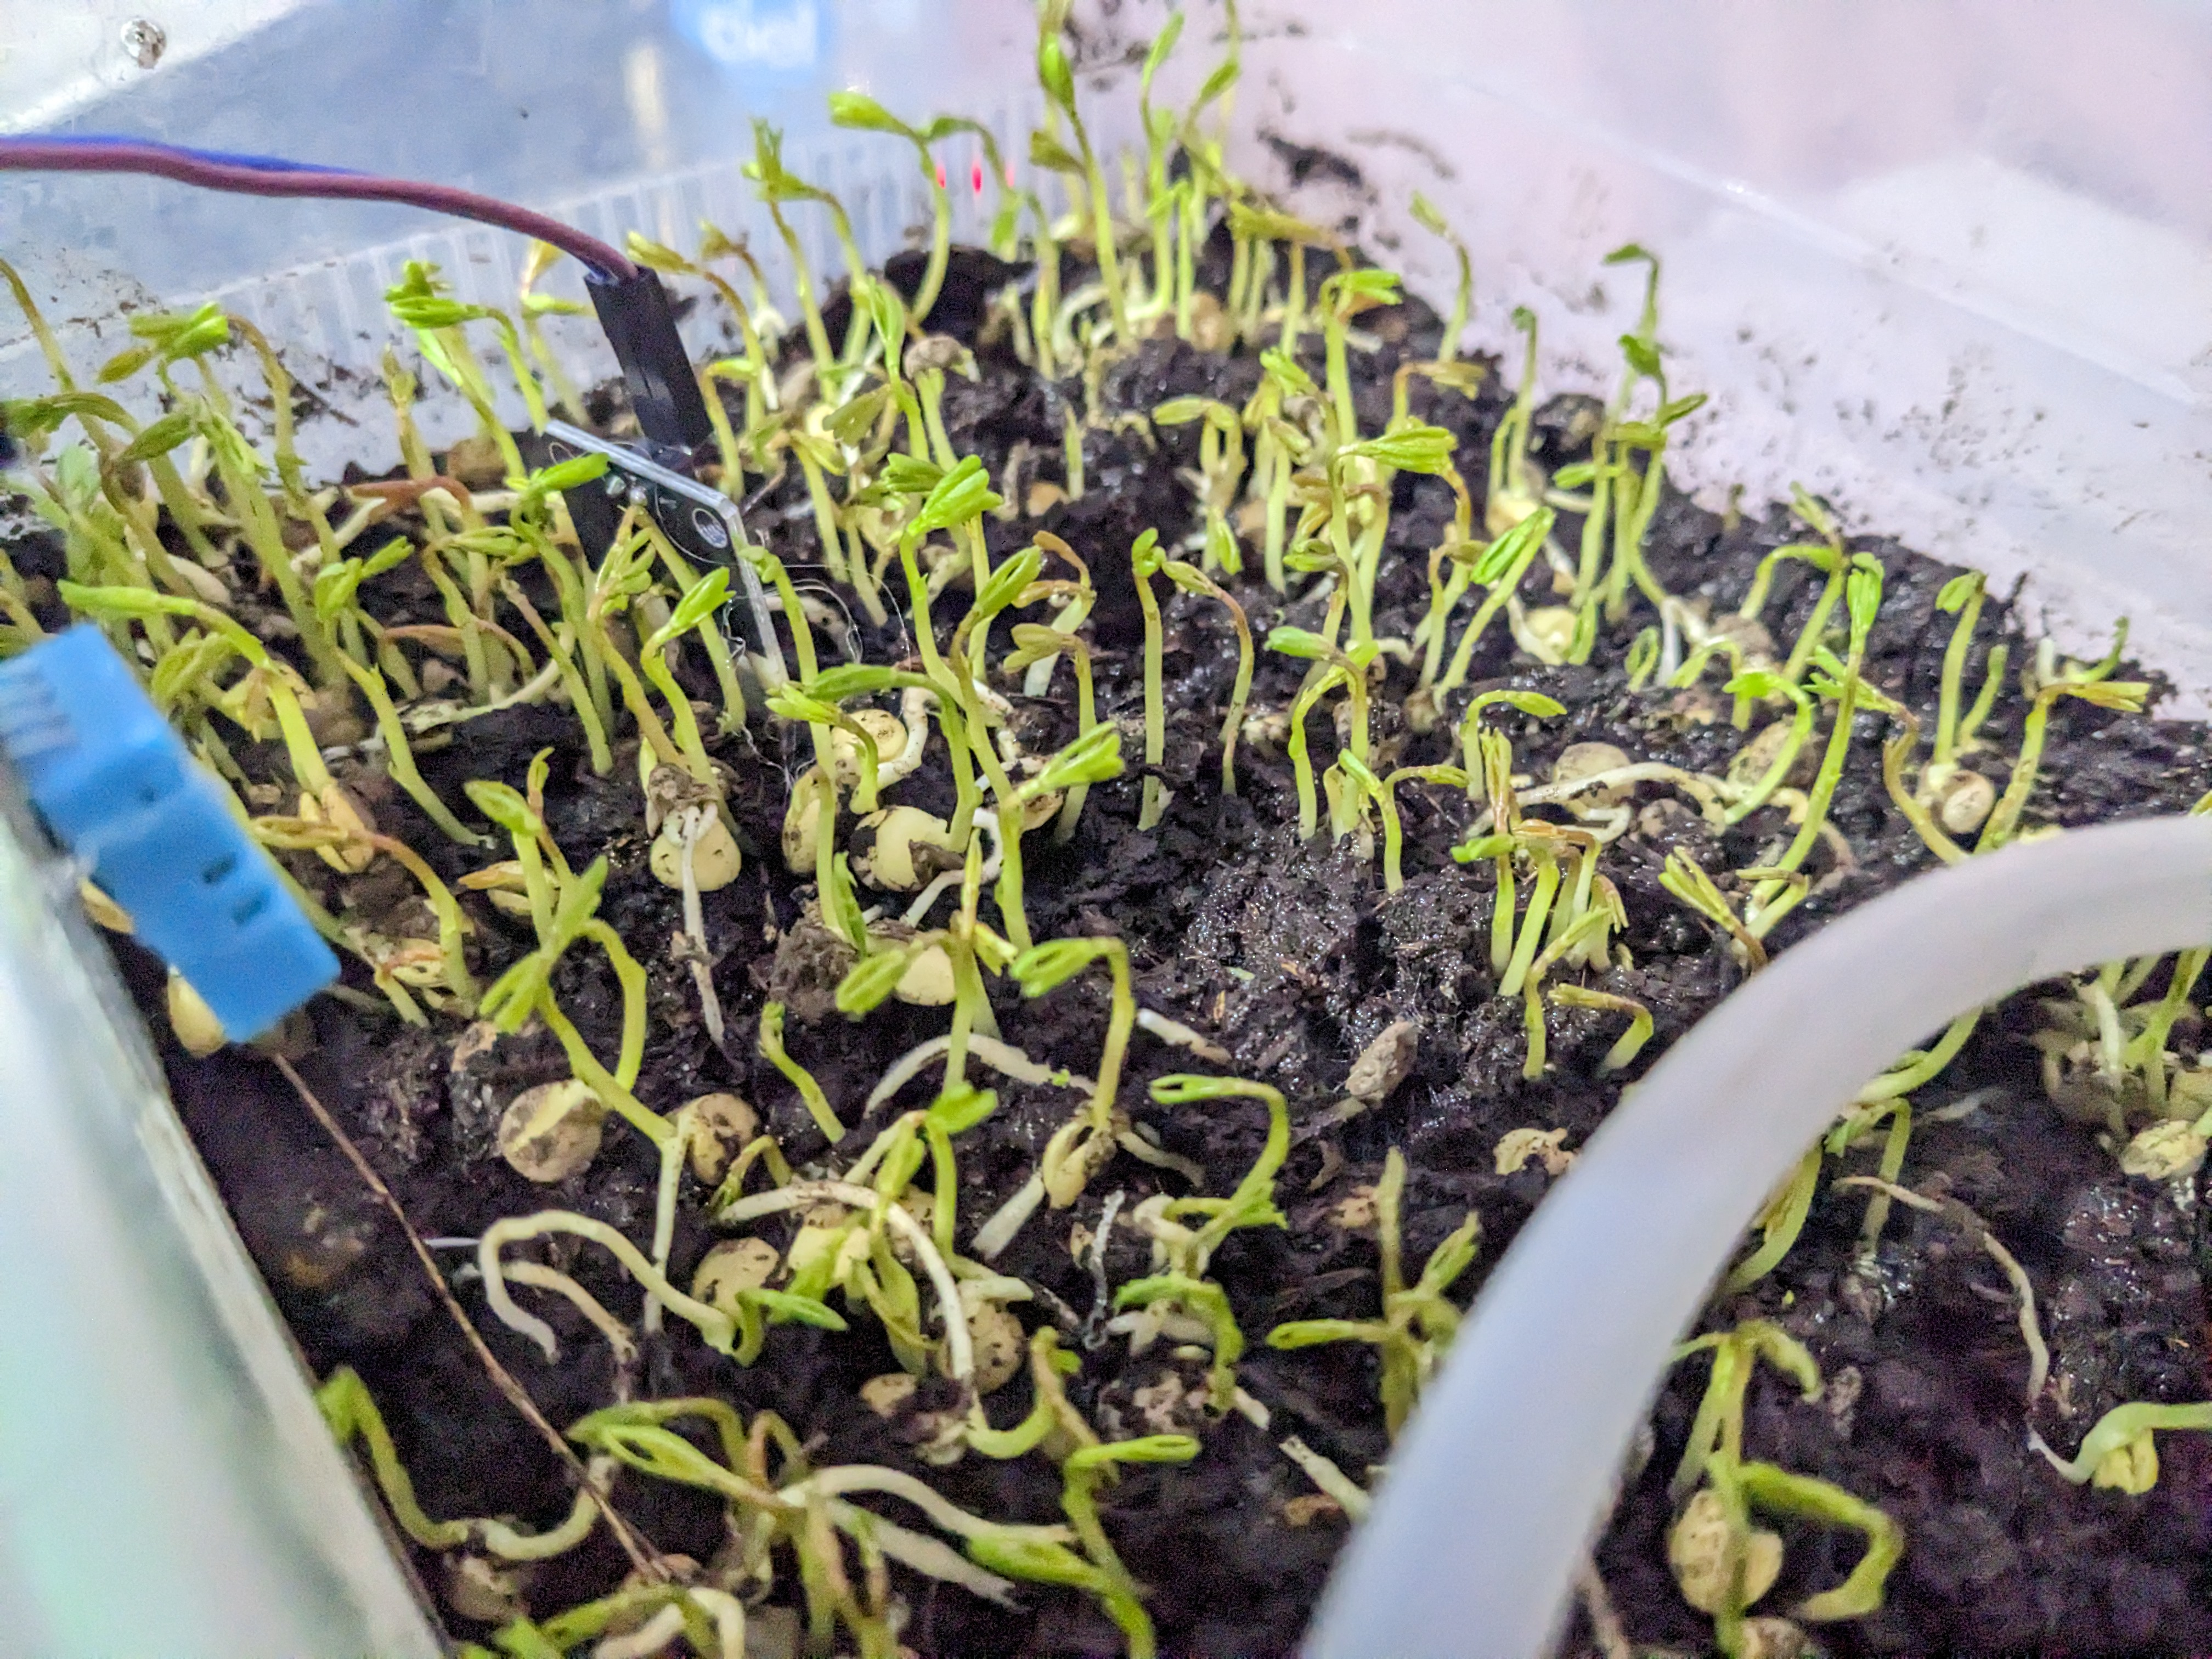
\includegraphics[width=\linewidth]{planta.jpg}
  \caption{Planta de lentejas que se cultivó con ayuda de Agrocare}
  \label{fig:example}
\end{figure}

También logramos proporcionar energía solar que ayudó a que el sistema sea autosustentable con una autonomía de aproximadamente 10 horas, suficiente para pasar la noche sin sol.